\documentclass[11pt,a4paper]{report}
\usepackage[utf8]{inputenc}
\usepackage[T1]{fontenc}
\usepackage[english]{babel}
\usepackage{amsmath,amsfonts,amssymb}
\usepackage{graphicx}
\usepackage{geometry}
\usepackage{fancyhdr}
\usepackage{float}
\usepackage{listings}
\usepackage{xcolor}
\usepackage{hyperref}
\usepackage{booktabs}
\usepackage{float}
\usepackage{caption}
\usepackage{subcaption}
\usepackage{enumitem}
\usepackage{url}

% Page geometry
\geometry{
    left=2.5cm,
    right=2.5cm,
    top=3cm,
    bottom=3cm
}

\setlength{\parindent}{0pt}

% Header and footer
\pagestyle{fancy}
\fancyhf{}
\fancyhead[L]{Homer Technical Report}
\fancyhead[R]{SCK CEN}
\fancyfoot[C]{\thepage}
\renewcommand{\headrulewidth}{0.4pt}

% Code listing style
\lstdefinestyle{pythonstyle}{
    language=Python,
    basicstyle=\ttfamily\small,
    keywordstyle=\color{blue}\bfseries,
    commentstyle=\color{gray},
    stringstyle=\color{red},
    numberstyle=\tiny\color{gray},
    numbers=left,
    stepnumber=1,
    numbersep=8pt,
    showstringspaces=false,
    breaklines=true,
    frame=single,
    backgroundcolor=\color{gray!10},
    captionpos=b
}

\lstset{style=pythonstyle}

% Hyperref setup
\hypersetup{
    colorlinks=true,
    linkcolor=blue,
    filecolor=magenta,
    urlcolor=cyan,
    pdftitle={Homer Technical Report},
    pdfauthor={Florent Bergé, Mathieu de la Barre},
    pdfsubject={RAG Application for Nuclear Reactor Documentation},
    pdfkeywords={RAG, AI, Nuclear, MYRRHA, LangGraph, ChromaDB}
}

% Title page information
\title{\textbf{Homer - Technical Report}}
\author{
    Florent Bergé \\
    \and
    Mathieu de la Barre \\
    \textit{IMT Atlantique}
}
\date{March 1st - July 18th, 2025}

\begin{document}

% Title page
\begin{titlepage}
    \centering
    \vspace*{2cm}
    
    {\huge\bfseries Homer - Technical Report\par}
    \vspace{1cm}
    {\Large\itshape A Retrieval-Augmented Generation System for Nuclear Engineers Documentation\par}
    \vspace{2cm}
    
    {\Large
    Florent Bergé \\
    Mathieu de la Barre \\
    \textit{IMT Atlantique}
    \par}
    \vspace{1cm}
    
    {\large Supervised by: Mr. Vincenzo De Florio\par}
    \vspace{2cm}
    
    {\large
    \textbf{SCK CEN} \\
    Belgian Nuclear Research Centre \\
    March 1st - July 18th, 2025
    \par}
    
    \vfill
    
    {\large
    Classification: Public
    \par}
    
\end{titlepage}

% Table of contents
\tableofcontents
\newpage

\section{Abstract}

This report presents the results of a research and development project conducted by Florent Bergé and Mathieu de la Barre, engineering trainees from IMT Atlantique, between March 1st and July 18th, 2025. The project focused on the design and implementation of Homer, a generative AI assistant tailored for the retrieval and interpretation of technical knowledge within the framework of the SMR-LFR nuclear reactor program at SCK CEN.

The work was carried out under the supervision of Mr. Vincenzo De Florio, and builds on existing specifications, which are assumed as prior knowledge for the reader. The report details both the conceptual foundations and the technical implementations of the assistant, from document analysis and vectorization strategies to evaluation protocols and system architecture. The resulting tool is expected to significantly improve information accessibility and decision-making efficiency for domain experts engaged in advanced nuclear research.

\section{Introduction}

The SCK CEN has progressively accumulated a substantial body of knowledge through its involvement in the MYRRHA program and, more recently, the SMR-LFR nuclear reactor initiative. This expertise has been systematically documented in the Conceptual Design Report (CDR), a dynamic reference work currently exceeding 3,500 pages, as well as in an extensive knowledge base of requirements, design rationales, and engineering constraints. These resources are managed within Polarion environments dedicated to Requirements and Configuration Management.

In light of the growing complexity and scale of these assets, SCK CEN has initiated an exploration into the use of generative AI technologies. The goal is to develop a reasoning assistant—akin to an expert system—that can support engineers in efficiently retrieving critical information related to MYRRHA and in navigating toward the most pertinent enterprise knowledge resources.

The result of this initiative is Homer, a multi-user assistant based on Retrieval-Augmented Generation (RAG) architecture. Designed as a secure, cloud-hosted solution within SCK CEN's infrastructure, it is tailored to respect the confidentiality and sensitivity of the internal documentation.

The name Homer pays homage to the ancient Greek poet traditionally regarded as the author of the Iliad and the Odyssey. In conceptual harmony with Alexandria—a symbolic reference to the accumulation and preservation of knowledge—Homer stands for its interpretation and transmission\cite{berge2025specifications}.

\newpage
\chapter{Concepts}

\section{Retrieval-Augmented Generation}

The Retrieval-Augmented Generation (RAG) pattern is an industry-standard approach to building applications that use language models to process specific or proprietary data that the model doesn't already know. The architecture is straightforward and best suited for large and fast-changing data sets (compared to fine-tuning).

\begin{figure}[H]
        \centering
        \includegraphics[width=1\linewidth]{static/schemas/query.png}
        \caption{RAG application flow}
        \label{fig:ragflow}
    \end{figure}

\begin{enumerate}
    \item The user issues a query
    \item The application performs a search on the vectorstore based on the user input
    \item The top k results matching the query are extracted. Both the results and the query are then packaged together in a prompt and sent to the Large Language Model (LLM)
    \item The LLM outputs a structured answer based on both the input and the retrieved context
\end{enumerate}

\section{Core Components}

\subsection{Vectorstore}
A vectorstore is a specialized database designed to store and retrieve high-dimensional vectors efficiently. In the context of RAG applications, vectorstores serve as the foundation for semantic search capabilities. They enable the system to find relevant documents based on meaning rather than exact keyword matches. The vectorstore indexes document embeddings and supports similarity searches using distance metrics such as cosine similarity, Euclidean distance, or dot product. Popular vectorstore solutions include Pinecone, Weaviate, Chroma, and FAISS, each offering different trade-offs between performance, scalability, and ease of deployment.

\subsection{Tokens, Embeddings and Embedding Models}
\textbf{Tokens} are the fundamental units of text that language models process. Text is broken down into tokens, which can represent words, subwords, or characters depending on the tokenization strategy. Modern models typically use subword tokenization methods like Byte Pair Encoding (BPE) or SentencePiece.

\textbf{Embeddings} are dense vector representations of text that capture semantic meaning in a high-dimensional space. Each embedding is a numerical array where semantically similar concepts are positioned closer together in the vector space. These embeddings enable the system to understand context and meaning beyond simple keyword matching.

\textbf{Embedding models} are specialized neural networks trained to convert text into these vector representations. Popular embedding models include OpenAI's text-embedding-ada-002, Sentence-BERT, and various models from Hugging Face's transformers library. The choice of embedding model significantly impacts the quality of document retrieval and overall system performance.

\subsection{Chat Model}
The chat model is the large language model responsible for generating responses in the RAG system. It receives both the user's query and the retrieved context documents as input, then synthesizes this information to produce coherent, contextually relevant answers. Common chat models include GPT-3.5/4, Claude, Llama, and other instruction-tuned language models. The chat model's performance depends on its ability to understand context, follow instructions, and generate accurate responses based on the provided information.

\section{Document Processing Pipeline}

\subsection{Indexing}
An indexing pipeline allows transforming files into useable data for the RAG application. The data pipeline processes each document individually by completing the following steps:

\begin{figure}[H]
        \centering
        \includegraphics[width=1\linewidth]{static/schemas/documentLoader.png}
        \caption{Indexing pipeline}
        \label{fig:indexpipeline}
\end{figure}

\begin{enumerate}
    \item \textbf{Loading}: Data is extracted from the documents
    \item \textbf{Chunking}: The document is divided into smaller parts—recommended between 256 and 512 chunks—according to a chunking technique
    \item \textbf{Chunk enrichment}: Adds metadata fields that the pipeline creates based on the content in the chunks, such as the source document, the titles and other relevant information
    \item \textbf{Indexing}: All the chunks are turned into embeddings and stored into a vector database according to an indexing algorithm\cite{berge2025hybrid}
\end{enumerate}

\subsection{Chunking Techniques}
The system supports two chunking approaches:

\textbf{Recursive Character Splitting}: The data is divided into chunks of a given size with specified overlap between adjacent chunks. The overlap prevents sentences from being split in the middle, which could potentially cause loss of meaning. This method provides consistent chunk sizes but may not preserve semantic boundaries.

\textbf{Semantic Text Chunking}: This technique requires an embedding model to divide content based on meaning rather than character count. It preserves most sentences or propositions intact and then combines semantically related chunks together. While more computationally expensive, this approach often results in more coherent and contextually meaningful chunks.

\section{Framework Architecture}

\subsection{LangChain Framework}
LangChain is a popular open-source framework designed to simplify the development of applications powered by large language models. It provides a comprehensive set of tools and abstractions that streamline the implementation of RAG systems by offering pre-built components, standardized interfaces, and seamless integrations with various LLMs, vector databases, and data sources. The framework follows a modular architecture that allows developers to mix and match components while maintaining clean, maintainable code.

\textbf{Key LangChain Components:}

\begin{itemize}
    \item \textbf{The Retriever}: A core abstraction that defines a standard interface for fetching relevant documents based on a query. It acts as the bridge between the user's question and the vectorstore, encapsulating the search logic and returning a list of relevant documents
    \begin{itemize}
        \item \textit{VectorStoreRetriever}: Performs similarity search on vector databases
        \item \textit{MultiQueryRetriever}: Generates multiple variations of the user query to improve retrieval coverage
    \end{itemize}
    
    \item \textbf{The Document Class}: LangChain's standardized representation of a piece of text content along with its associated metadata. Each Document object contains:
    \begin{itemize}
        \item \textit{page\_content}: The actual text content of the document chunk
        \item \textit{metadata}: A dictionary containing additional information such as source file, page number, creation date, document type, and custom fields
    \end{itemize}
\end{itemize}

\subsection{LangGraph}
LangGraph is a framework built on top of LangChain that enables the creation of stateful, multi-actor applications with large language models. It represents a paradigm shift from simple linear chains to complex, graph-based workflows where different components can interact, make decisions, and maintain state over time. LangGraph is particularly valuable for RAG applications that require sophisticated orchestration, conditional logic, human-in-the-loop workflows, or multi-step reasoning processes.

\textbf{Core LangGraph Components:}

\begin{itemize}
    \item \textbf{The Graph}: The core abstraction that defines the structure and flow of your application. It represents a directed graph where nodes perform specific tasks and edges define the transitions between these tasks;
    \item \textbf{Nodes}: Individual processing units within a LangGraph. Each node encapsulates a specific function, receiving the current state as input and returning updated state information;
    \item \textbf{State Management}: Allows information to persist and evolve throughout the execution of a graph. The state serves as a shared data structure that nodes can read from and write to;
    \item \textbf{The Checkpointer}: Responsible for persisting the state of a graph execution at specific points, enabling durability and recovery capabilities. In our implementation, we use an in-memory SQLite database;
    \begin{lstlisting}[caption={Checkpointer usage}]
from langgraph.checkpoint.sqlite import SqliteSaver

builder = StateGraph(...

conn = sqlite3.connect(':memory:', check_same_thread=False)
memory = SqliteSaver(conn)

graph = builder.compile(checkpointer=memory)
    \end{lstlisting}
    \item \textbf{The Runnable Config}: A configuration object that controls how a graph executes, providing fine-grained control over the execution environment and allowing configuration to be passed inside the nodes. In order to provide a custom configuration to the graph, it needs to be passed in the "configurable" argument of the RunnableConfig and turned into a dictionary. To use a checkpoint, you also have to add a \textit{thread\_id} to the configurable dictionary;
    \begin{lstlisting}[caption={Runnable config usage}]
configuration = {"parameter1":value1, ...}|{"thread_id":1}

graph.invoke(
    input=user_input,
    config={"configurable":configuration}
)
    \end{lstlisting}
\end{itemize}

\chapter{Architecture}

Homer is a RAG application that allows users to provide their own documents to augment the agent's knowledge. It is composed of a Streamlit web interface, LangGraph agents, and an Ollama client.

\begin{figure}[H]
    \centering
    \includegraphics[width=0.5\linewidth]{static/schemas/scope.png}
    \label{fig:scope}
\end{figure}

The core Application (interface, agents and vectorstore) runs on the local machine and sends requests to an Ollama client which handles model inferences. The latter can either be running on the local machine as well or on a distant server.

This architecture was chosen because it allows confidential data to stay on the local machine. Indeed, having a shared database between users would have required either managing the access of each user to specific documents or creating user-specific spaces which would have caused redundancy. Hence, the decision was made to perform all small calculations on the local computer and let a server run the models using the Ollama API.

\section{Code architecture}

\begin{figure}[H]
    \centering
    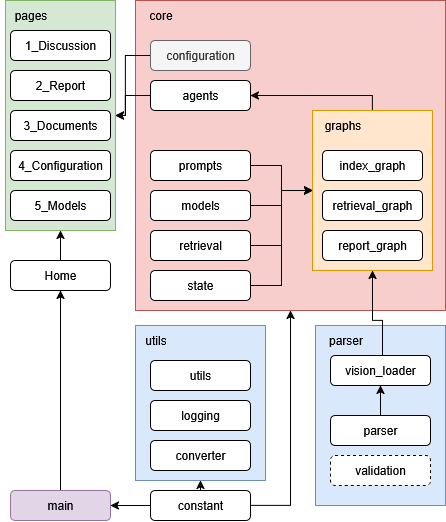
\includegraphics[width=0.7\linewidth]{static/schemas/projectOverview.drawio.png}
    \caption{Code organization}
    \label{fig:overview}
\end{figure}

The application starts by running:

\begin{lstlisting}
python main.py
\end{lstlisting}

This file ensures mandatory directories exist and then runs the line:

\begin{lstlisting}
streamlit run streamlit_app.py
\end{lstlisting}

\begin{itemize}
    \item \textbf{Pages} refers to the streamlit interface pages, which are managed by the file \texttt{streamlit\_app}
    \item \textbf{core} refers to the core components (configuration and agents related files)
    \item \textbf{utils} are all the utility functions that can be called in any file, such as the log management, functions to load a sqlite3 connection etc
    \item \textbf{parser} refers to the custom pdf parser described in Chapter 3
\end{itemize}

\section{Streamlit Client}

The Streamlit client is composed of 6 pages:

\begin{itemize}
    \item \textbf{Home}: Welcome page with navigation
    \item \textbf{Discussion}: The page where users can chat with the RetrievalAgent
    \item \textbf{Report}: The page where users can send a query to the ReportAgent
    \item \textbf{Documents}: The page to add documents to the knowledge base
    \item \textbf{Configuration}: The page where users can temporarily modify parameters
    \item \textbf{Models}: Allows users to enter an Ollama model to pull
\end{itemize}

\subsection*{Session state}

Streamlit uses a 'session\_state' to store session variables such as:

\begin{itemize}
    \item \textbf{baseConfig} (Configuration): Loads the default Configuration
    \item \textbf{ollama\_host} (str): The IP address of the distant Ollama client
    \item \textbf{models} (dictionary): The discussion models, reasoning or standard, local or server (server ones are larger and more accurate than local ones)
\end{itemize}

\subsection{Discussion Page}

\begin{figure}[H]
    \centering
    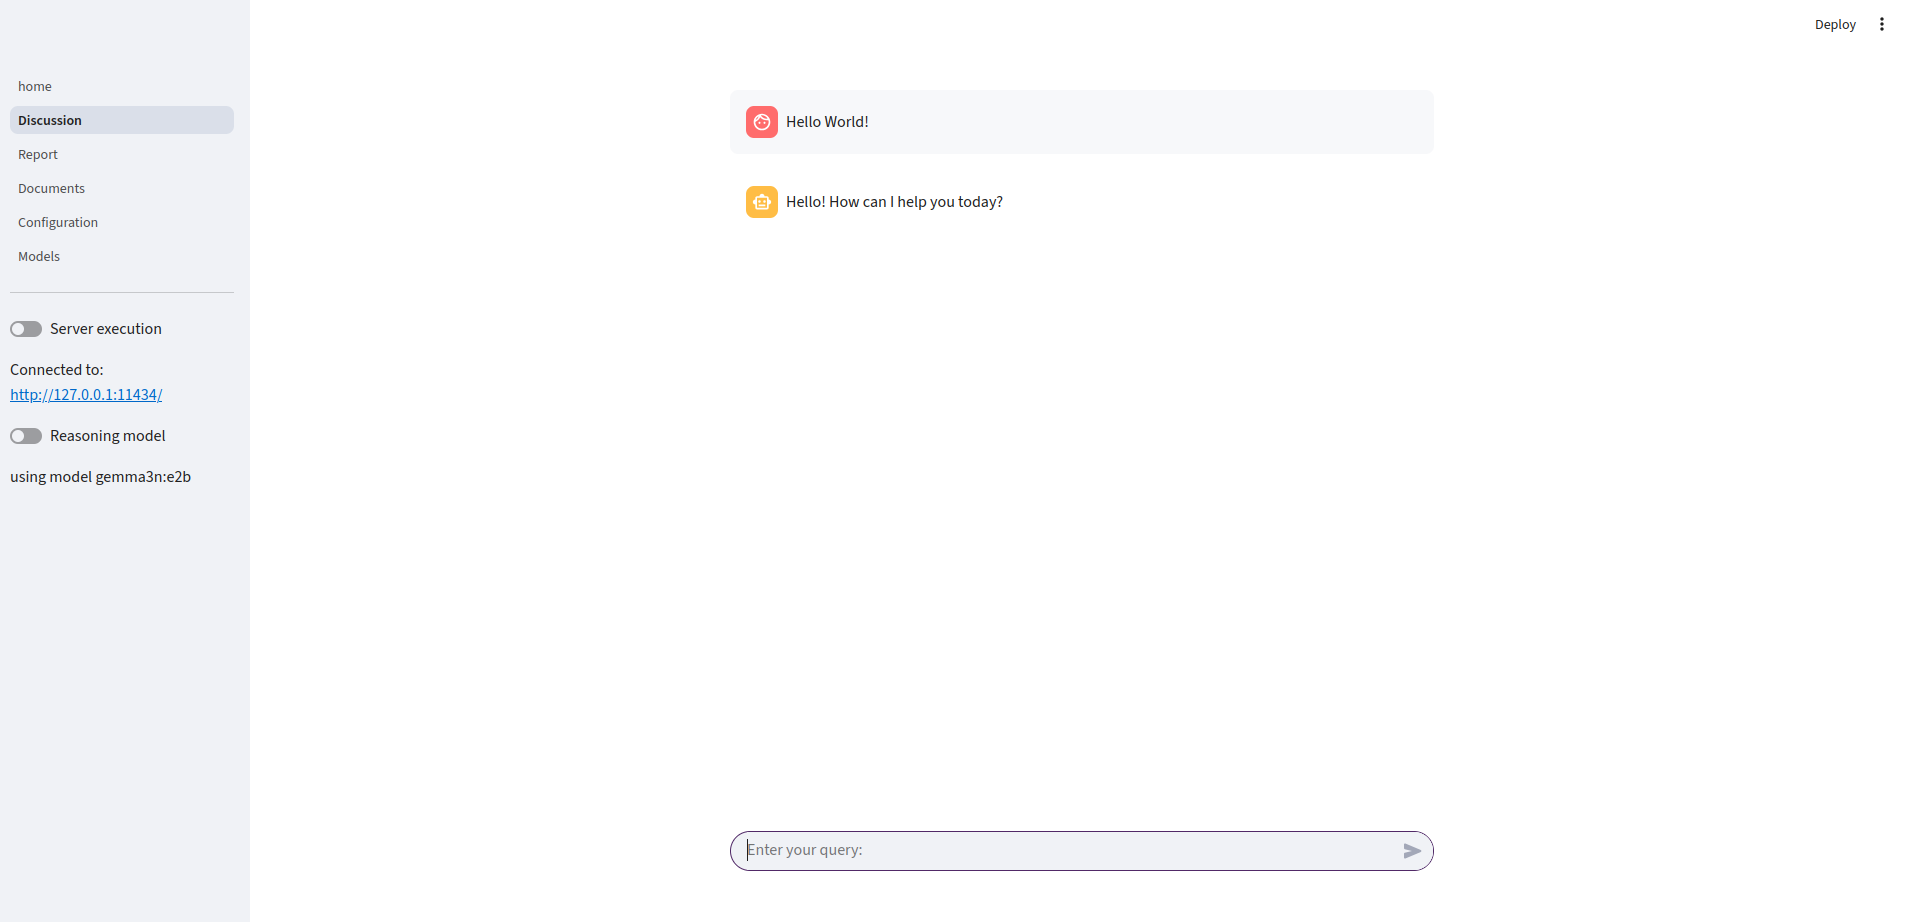
\includegraphics[width=1\linewidth]{static/figures/discussionPage.png}
    \label{fig:discussionPage}
\end{figure}

This is the main page for asking questions to the RetrievalAgent. The discussion displays in the main page, above the input field at the bottom. It features 2 buttons in the sidebar:

\begin{itemize}
    \item \textbf{Server Execution}: Allows running models on the distant client at the 'ollama\_host' address, if available
    \item \textbf{Reasoning Model}: Allows switching between traditional and reasoning models. Due to their 'thinking' step, they take more time to output an answer. When Reasoning model is on, the thinking part will be accessible through an expander on top of the answer
\end{itemize}

The specific session\_state values for this page are:
\begin{itemize}
    \item \textbf{retrievalAgent} (RetrievalAgent): The compiled retrieval agent
    \item \textbf{ollama\_host}
    \item \textbf{baseConfig}
    \item \textbf{models}
\end{itemize}

Loading the retrieval agent in the session\_state allows compiling the graph only once.

\subsection{Report Page}

\begin{figure}[H]
    \centering
    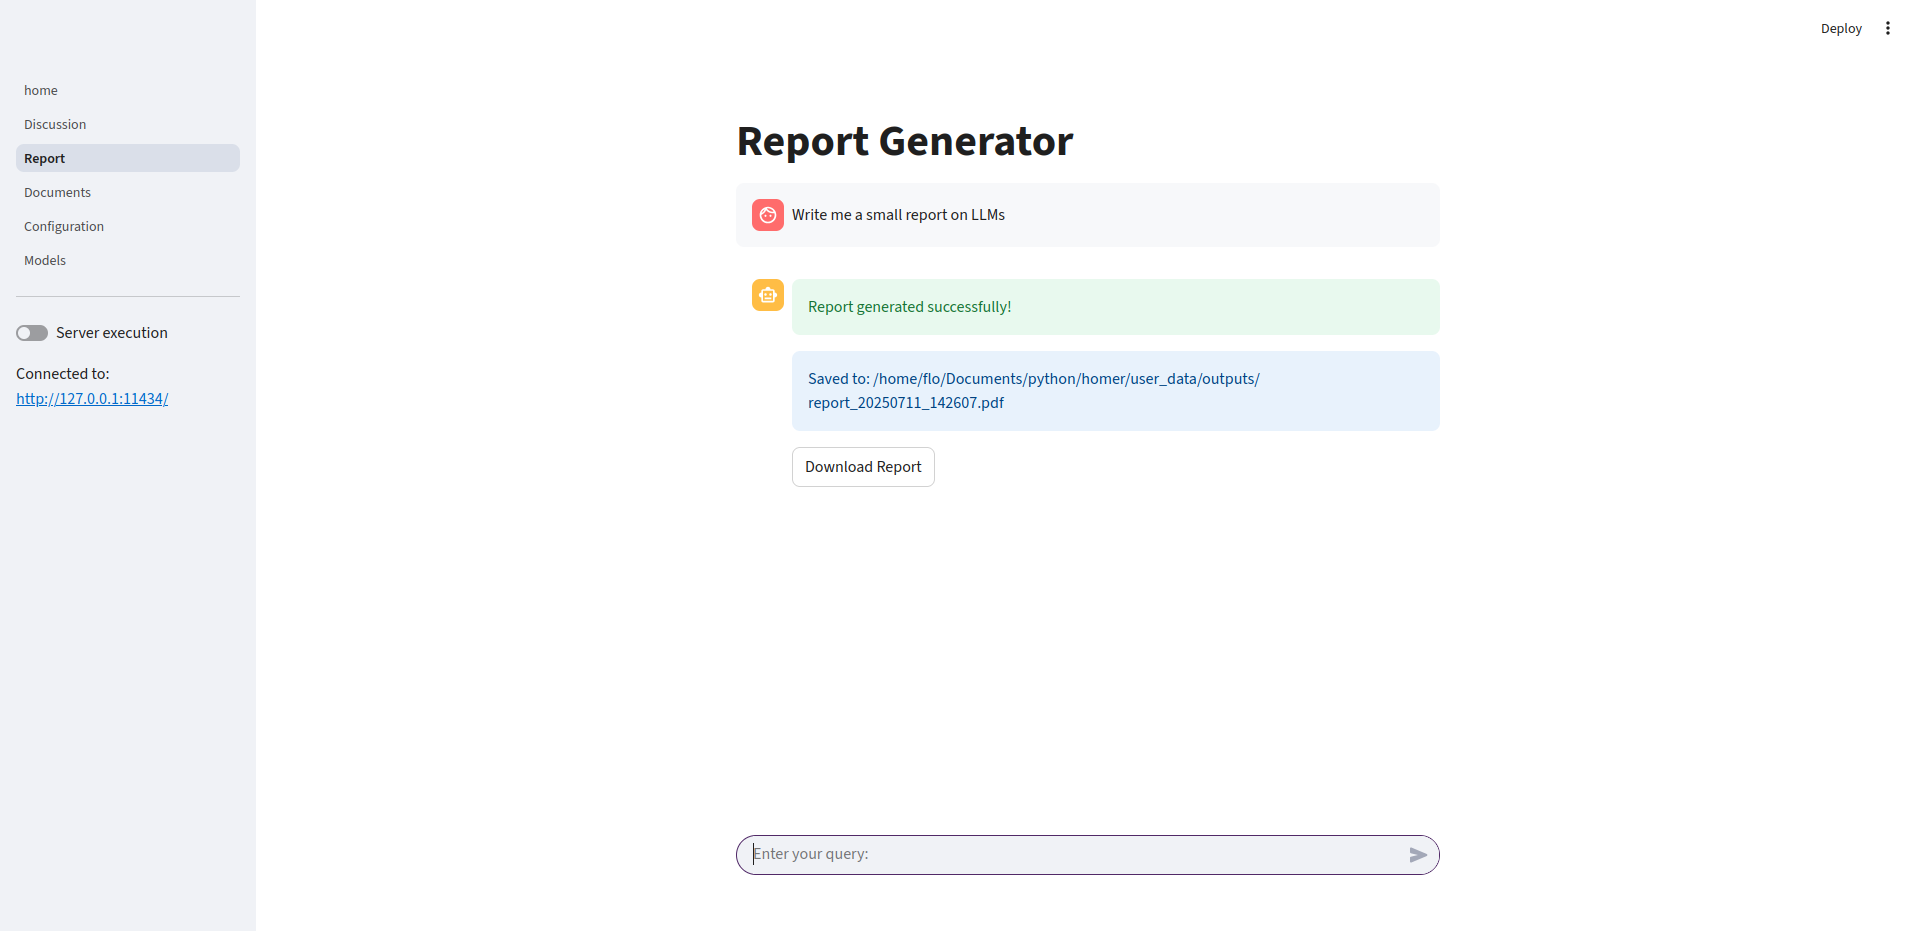
\includegraphics[width=1\linewidth]{static/figures/reportPage.png}
    \label{fig:reportPage}
\end{figure}

This page allows the user to request a report to the ReportAgent. The sidebar features 2 options:

\begin{itemize}
    \item \textbf{Server Execution}
    \item \textbf{Writing}: Allows switching between 'general' and 'technical' writing style
\end{itemize}

Once a report is completed, a button to download it.

The specific session\_state values for this page are:
\begin{itemize}
    \item \textbf{reportAgent} (ReportAgent): The compiled report agent
    \item \textbf{report\_history} (list): A list of previous reports from the session
    \item \textbf{ollama\_host}
    \item \textbf{baseConfig}
\end{itemize}

\subsection{Document Page}

\begin{figure}[H]
    \centering
    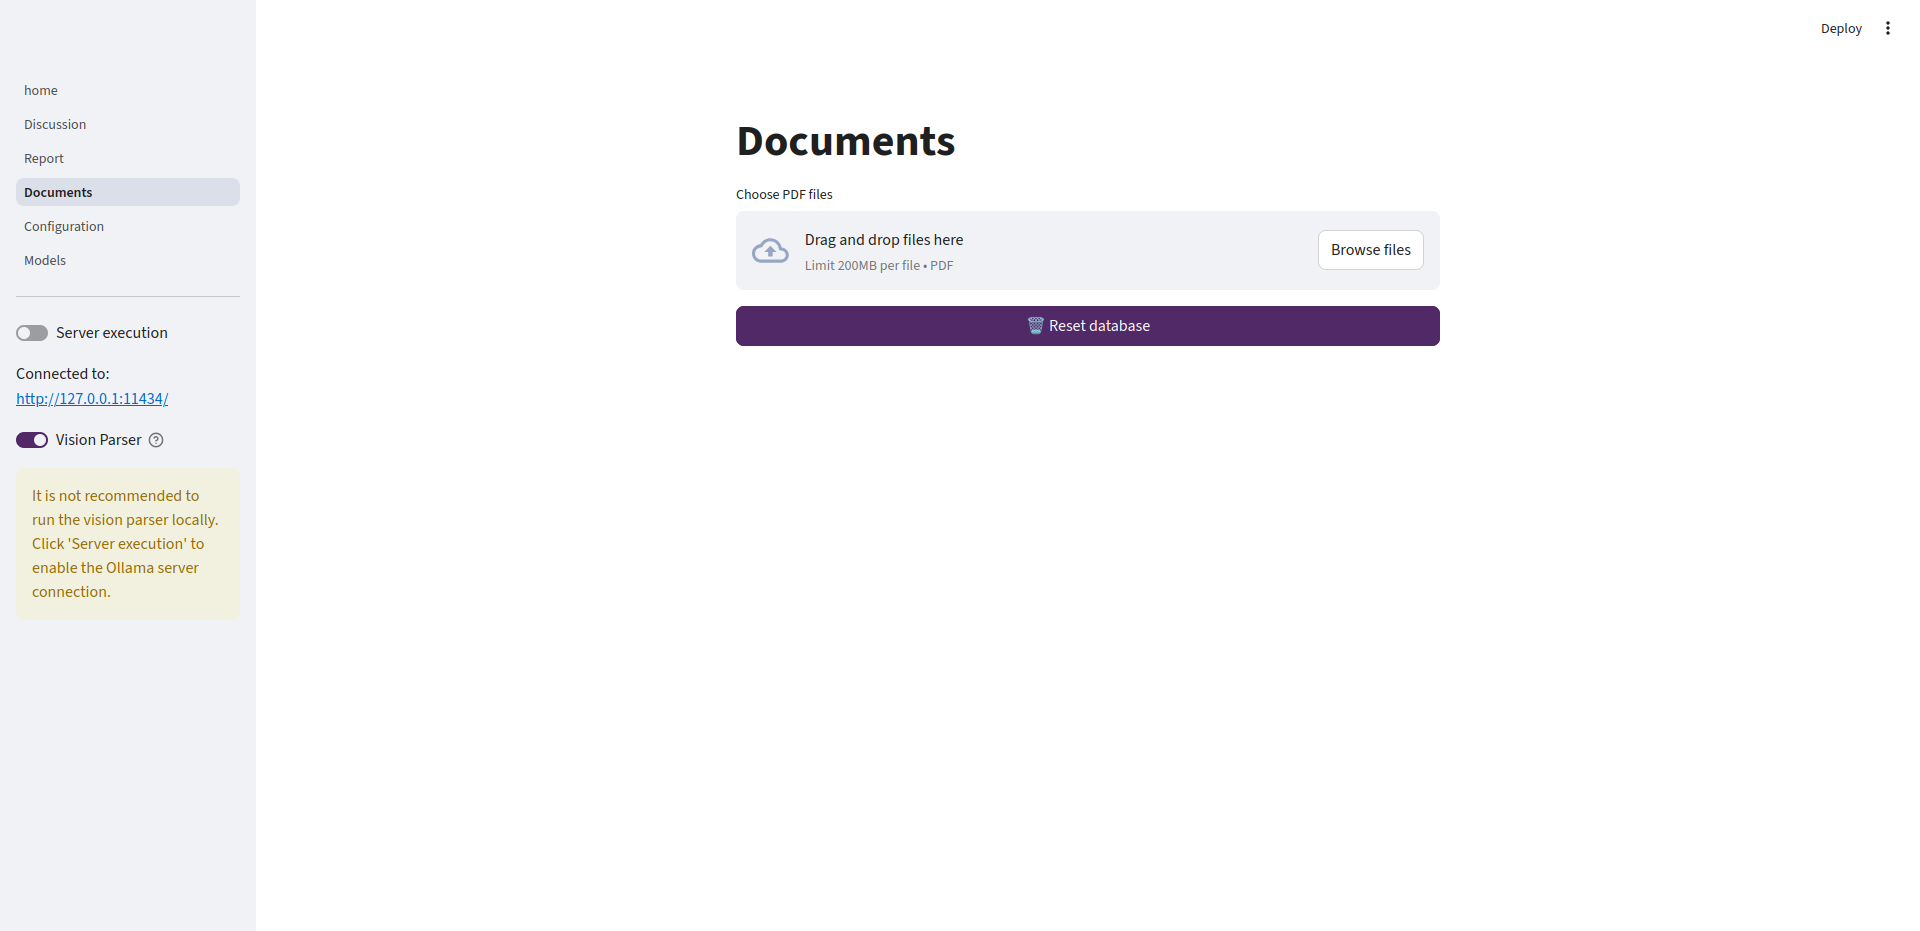
\includegraphics[width=\linewidth]{static/figures/documentPage.png}
    \label{fig:documentPage}
\end{figure}

This page allows the user to send documents to the documents pipeline (IndexAgent). The sidebar features 2 options:

\begin{itemize}
    \item \textbf{Server Execution}
    \item \textbf{Vision parser}: Allows switching between PyMuPDF parser and a custom Vision parser (using a LLVM)
\end{itemize}

The specific session\_state values for this page are:
\begin{itemize}
    \item \textbf{indexAgent} (IndexAgent): The compiled indexing pipeline
    \item \textbf{ollama\_host}
    \item \textbf{baseConfig}
\end{itemize}

\subsection{Model Page}

\begin{figure}[H]
    \centering
    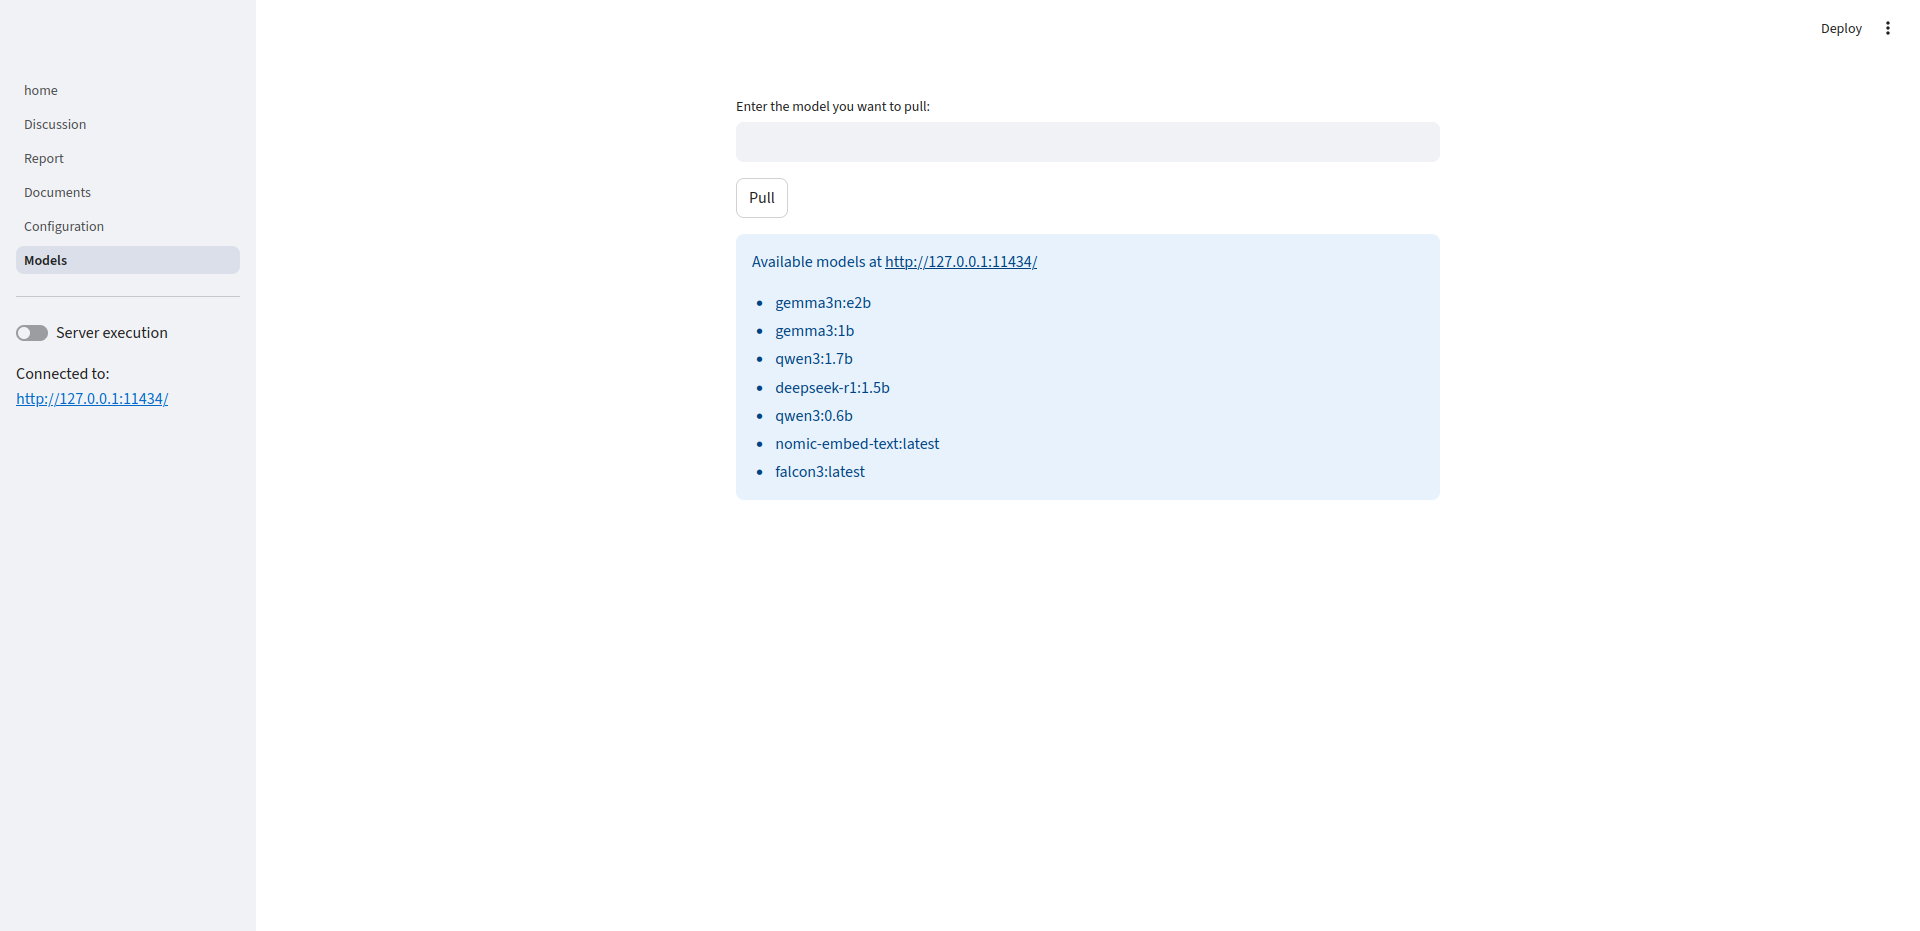
\includegraphics[width=\linewidth]{static/figures/modelPage.png}
    \label{fig:modelPage}
\end{figure}

This page allows the user to pull a model to either the local or server ollama client.

\section{Configuration Management}

\begin{figure}[H]
    \centering
    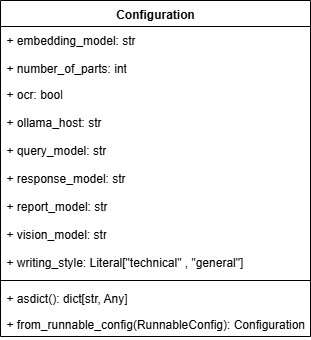
\includegraphics[width=0.5\linewidth]{static/schemas/classDiagramConfiguration.drawio.png}
    \label{fig:configuration}
\end{figure}

\subsection{Configuration Architecture}

Homer implements a centralized configuration system through the \texttt{Configuration} dataclass located in \texttt{src/core/configuration.py}. This approach ensures type safety, validation, and consistent parameter management across all system components.

The configuration system utilizes Python's \texttt{dataclass} decorator with the \texttt{kw\_only=True} parameter, enforcing explicit parameter naming and improving code readability. The implementation supports both static default values and dynamic configuration loading based on Ollama client availability.

\begin{lstlisting}[caption={Configuration dataclass structure}]
@dataclass(kw_only=True)
class Configuration:
    # Report configuration
    number_of_parts: int = field(default=5)
    
    # Ollama configuration  
    ollama_host: str = field(default=OLLAMA_LOCALHOST)
    
    # Model specifications
    embedding_model: str = field(default="nomic-embed-text")
    response_model: str = field(default="gemma3:1b")
    # ... additional model configurations
\end{lstlisting}

\subsection{Dynamic Host Resolution}

The system implements intelligent host resolution through the \texttt{\_is\_ollama\_client\_available()} function, which performs connectivity checks with a 2-second timeout. When the remote Ollama client at \texttt{OLLAMA\_CLIENT} is available, the configuration automatically switches to server execution mode. Otherwise, it falls back to local execution using \texttt{OLLAMA\_LOCALHOST} (\texttt{http://127.0.0.1:11434/}).

This dual-mode operation enables:
\begin{itemize}
    \item \textbf{Local development} with reduced model capabilities but full functionality
    \item \textbf{Production deployment} with access to larger, more capable models on dedicated hardware
    \item \textbf{Automatic failover} ensuring system availability regardless of server status
\end{itemize}

\subsection{Configuration Integration with LangGraph}

The configuration system integrates seamlessly with LangGraph's \texttt{RunnableConfig} through the \texttt{from\_runnable\_config()} class method. This enables:

\begin{lstlisting}[caption={Configuration integration with LangGraph}]
configuration = Configuration.from_runnable_config(config)
configurable = config.get("configurable") or {}
\end{lstlisting}

Each graph node receives configuration parameters through the standardized LangGraph configuration mechanism, ensuring consistent behavior across all agents and maintaining separation of concerns between business logic and configuration management.

\subsection{Model Selection Strategy}

Homer implements a sophisticated model selection strategy supporting four distinct model categories. These are the defaults:

\begin{table}[H]
\centering
\begin{tabular}{@{}llll@{}}
\toprule
\textbf{Category} & \textbf{Local Model} & \textbf{Server Model} & \textbf{Use Case} \\
\midrule
Standard & \texttt{gemma3n:e2b} & \texttt{gemma3:4b-it-qat} & General responses \\
Reasoning & \texttt{qwen3:0.6b} & \texttt{qwen3:30b-a3b} & Complex analysis \\
Embedding & \texttt{nomic-embed-text} & \texttt{nomic-embed-text} & Document vectorization \\
Vision & N/A & \texttt{qwen2.5vl:3b-q4\_K\_M} & PDF parsing with OCR \\
\bottomrule
\end{tabular}
\caption{Model selection strategy across different categories}
\label{tab:model-selection}
\end{table}

These values can be modified in the \texttt{src/pages/discussion.py} file.

The reasoning models incorporate a \texttt{<think>...</think>} mechanism, enabling explicit reasoning steps that are displayed separately from the final response in the user interface.

\section{Agents architecture}

Agents are organised as shown:

\begin{figure}[H]
    \centering
    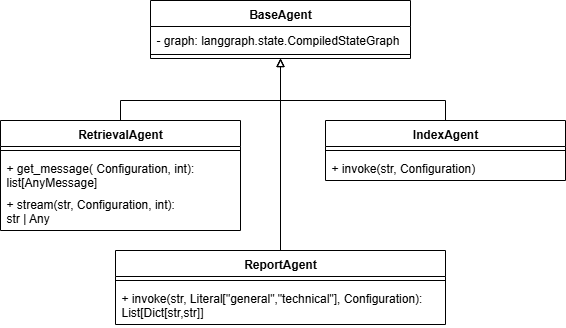
\includegraphics[width=\linewidth]{static/schemas/classDiagramAgents.drawio.png}
    \caption{Agents class diagram}
    \label{fig:agents}
\end{figure}

The \texttt{RetrievalAgent} and \texttt{ReportAgent} both use custom structured output at some point in their execution. They come in the form of pydantic's BaseModels:

\begin{figure}[H]
    \centering
    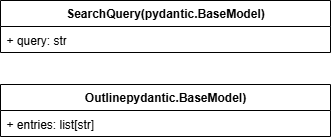
\includegraphics[width=0.5\linewidth]{static/schemas/classDiagramStructuredOutputs.drawio.png}
    \label{fig:StructuredOutputs}
\end{figure}

\subsection{Graph State Architecture}

Homer implements a sophisticated state management system using LangGraph's state abstractions. Each agent maintains its specific state structure while sharing common interfaces:

\begin{figure}[H]
    \centering
    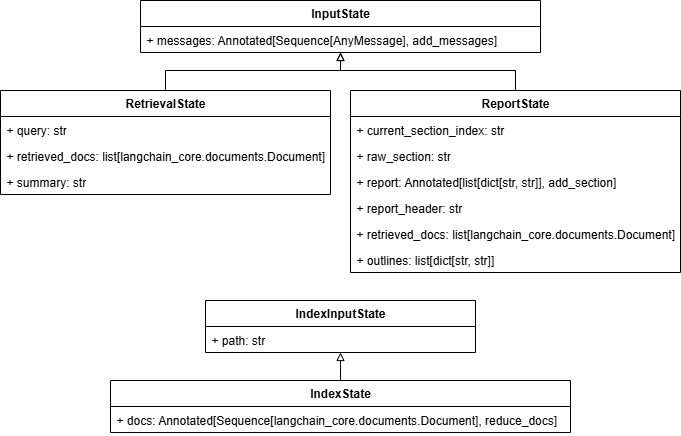
\includegraphics[width=\linewidth]{static/schemas/classDiagramStates.drawio.png}
    \caption{Agents states}
    \label{fig:states}
\end{figure}

\subsection{State Reducers}

The system implements custom state reducers for complex state transitions:

\begin{lstlisting}[caption={Document state reducer}]
def reduce_docs(existing: Optional[Sequence[Document]], 
                new: Union[Sequence[Document], str, Literal["delete"]]):
    if new == "delete":
        return []
    # Handle various input types and transformations
\end{lstlisting}

\subsection{Memory and Persistence}

\begin{itemize}
    \item \textbf{Conversation Memory}: RetrievalAgent uses SQLite-based checkpointing for conversation persistence
    \item \textbf{Document Storage}: ChromaDB provides persistent vector storage with metadata
    \item \textbf{Session State}: Streamlit manages user session state for UI consistency
\end{itemize}

In a previous version, making the discussions persistent has been considered, but the streamlit interface made switching discussions difficult. You can find some files related to this in \texttt{src/schemas} and \texttt{src/core/database.py}.\\
To enable the persistent database, the value \texttt{":memory:"} from \texttt{src/utils/utils.py, get\_connection} should be changed to the persistent database directory. It will not work out of the box as some functions related to this have been removed of the current release.

\subsection{RetrievalAgent - Conversational RAG Implementation}

The RetrievalAgent implements a stateful conversational retrieval system using LangGraph's state management capabilities. The agent maintains conversation context through an SQLite checkpointer, enabling multi-turn conversations with persistent memory.

\begin{figure}[H]
    \centering
    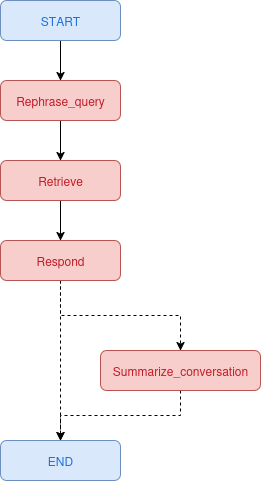
\includegraphics[width=0.4\linewidth]{static/schemas/retrievalGraph.drawio.png}
    \caption{Retrieval graph structure}
    \label{fig:retrievalGraph}
\end{figure}

\textbf{Nodes:}\\

\paragraph{Rephrase query}

Generate an optimized search query based on conversation context.  This function analyzes the current conversation state and generates a search query optimized for document retrieval, based on the last interaction.

\begin{lstlisting}[caption={Rephrase query node}]
def rephrase_query(
    state: RetrievalState, *, config: RunnableConfig
) -> Dict[str, Union[str, List]]:

    configuration = Configuration.from_runnable_config(config)
    
    # Load and configure model
    model = load_chat_model(
        model=configuration.query_model, 
        host=configuration.ollama_host
    ).with_structured_output(SearchQuery)
    
    # Prepare message context
    previous_messages = (
        format_messages(state.messages[-3:-1]) 
        if len(state.messages) >= 3 
        else "There were no previous messages."
    )
    
    # Create prompt
    system_prompt = prompts.REPHRASE_QUERY_SYSTEM_PROMPT.format(
        previous_messages= previous_messages,
    )
    user_prompt = state.messages[-1].content
    
    messages = [
        ("human", combine_prompts(system_prompt,user_prompt)),
    ]
    
    # Generate rephrased query
    generated = cast(SearchQuery, model.invoke(messages, config))
    
    retrievalAgentLogger.info(f"Generated query: '{generated.query}'")
    
    return {
        "query": generated.query,
        "retrieved_docs": "delete" if state.retrieved_docs else [],
    }
\end{lstlisting}

\paragraph{Retrieve}

Retrieve relevant documents based on the generated query. This function takes a search query from the state and retrieves the most relevant documents from the indexed document collection using vector similarity search. It uses the configured embedding model to encode the query and find matching documents.

\begin{lstlisting}[caption={Retrieve node}]
def retrieve(
    state: RetrievalState, *, config: RunnableConfig
) -> Dict[str, List[Document]]:

    configuration = Configuration.from_runnable_config(config)
    
    # Load embedding model
    embeddings = load_embedding_model(
        model=configuration.embedding_model, 
        host=configuration.ollama_host
    )

    # Retrieve documents
    with retrieval.make_retriever(embedding_model=embeddings) as retriever:
        response = retriever.invoke(state.query, config)
        
        if response:
            retrievalAgentLogger.info(f"Successfully retrieved {len(response)} documents")
            for doc in response:
                retrievalAgentLogger.debug(f"Document: {doc.page_content} from {doc.metadata.get('source', 'unknown')}\n")
        else:
            retrievalAgentLogger.warning("No documents retrieved for the query")
        
        return {"retrieved_docs": response}
\end{lstlisting}

\paragraph{Respond}

 Generate a conversational response based on retrieved documents and chat history. This function creates a contextual response using the retrieved documents as context, considering the conversation history and any existing conversation summary. It handles message history efficiently by using summaries for older conversations.

\begin{lstlisting}[caption={Respond node}]
def respond(
    state: RetrievalState, *, config: RunnableConfig
) -> Dict[str, Union[List[BaseMessage], List, str]]:

    configuration = Configuration.from_runnable_config(config)
    
    # Load model
    model = load_chat_model(
        model=configuration.response_model, 
        host=configuration.ollama_host
    )
    
    # Prepare context
    previous_messages = ya_format_messages(state.messages[-3:-1] if len(state.messages)>2 else [])
    context_docs = format_docs(state.retrieved_docs) if state.retrieved_docs else ""
    
    # Create prompt
    system_prompt = prompts.RESPONSE_SYSTEM_PROMPT.format(
        context = context_docs,
        summary = state.summary if state.summary else "",
    )

    messages = [
        ("system", system_prompt)
    ] + previous_messages + [
        ("human", state.messages[-1].content)
    ]

    # Generate response
    response = model.invoke(input=messages, config=config)

    return {
        "messages": [response],
        "retrieved_docs": [],
        "query": "",
    }
\end{lstlisting}

\paragraph{Summarize conversation}

Create or extend a conversation summary to manage long chat histories. This function generates a concise summary of recent conversation messages, either creating a new summary or extending an existing one. This helps maintain context while keeping prompt sizes manageable for long conversations.
    
\begin{lstlisting}[caption={Summarize conversation node}]
def summarize_conversation(
    state: RetrievalState, *, config: RunnableConfig
) -> Dict[str, str]:

    configuration = Configuration.from_runnable_config(config)
    
    # Get existing summary
    existing_summary = state.summary if state.summary else ""
    messages_to_summarize = ya_format_messages(state.messages[-6:])  # Last 6 messages
    
    # Determine prompt based on existing summary
    if existing_summary:
        summary_system_prompt = f"""This is summary of the conversation to date:
<summary>
{existing_summary}
</summary>

Extend the summary by taking into account the new messages:"""

    else:
        summary_system_prompt = "Create a summary of the conversation:"

    # Load model
    model = load_chat_model(
        model=configuration.query_model, 
        host=configuration.ollama_host
    )
    
    # Create prompt
    messages = [
        ('system', summary_system_prompt)
    ] + messages_to_summarize

    
    response = model.invoke(messages, config)

    return {"summary": response.content}
\end{lstlisting}

Determine whether conversation summarization should occur. This function implements the logic for deciding when to summarize the conversation based on message count. It triggers summarization every 6 messages to keep conversation context manageable while preserving important information.
    
\begin{lstlisting}[caption={Summarize conditional edge}]
def should_summarize(
    state: RetrievalState, *, config: RunnableConfig
) -> str:
    message_count = len(state.messages)
    should_trigger = message_count % 6 == 0

    if should_trigger:
        return "summarize_conversation"
    else:
        return END
\end{lstlisting}

\subsection{ReportAgent - Structured Document Generation}

The ReportAgent generates comprehensive technical reports through a multi-stage pipeline that creates structured, well-organized documents from the knowledge base.

\begin{figure}[H]
    \centering
    \includegraphics[width=0.2\linewidth]{static/schemas/reportGraph.drawio.png}
    \caption{Report graph structure}
    \label{fig:reportGraph}
\end{figure}

\textbf{Nodes:}\\

\paragraph{Initial retrieval}

Retrieve documents based on the input state to create the outline. This function performs the initial document retrieval using the user's main query to gather relevant context that will inform the outline generation. It serves as the foundation for understanding what information is available for the report.

\begin{lstlisting}[caption={Initial retrieval node}]
def initial_retrieval(
    state: ReportState, *, config: RunnableConfig) -> dict[str, list[Document]]:

    configuration = Configuration.from_runnable_config(config)
    
    # Extract main query from the last message
    main_query = get_message_text(state.messages[-1])

     # Setup retriever with embedding model
    with retrieval.make_retriever(
        embedding_model=load_embedding_model(model=configuration.embedding_model, host=configuration.ollama_host),   
    ) as retriever:
        # Perform document retrieval
        response = retriever.invoke(main_query, config)
        
    return {"retrieved_docs": response}
\end{lstlisting}

\paragraph{Generate outline}

Generate an outline based on the user query and retrieved context. This function creates a structured outline for the report using the initially retrieved documents as context. It uses a language model with structured output to ensure the outline has the proper format and number of sections specified in the report configuration.

\begin{lstlisting}[caption={Initial retrieval node}]
def generate_outline(
    state: ReportState, *, config: RunnableConfig) -> dict[str, Any]:

    configuration = Configuration.from_runnable_config(config)
    
    # Extract query and context information
    main_query = get_message_text(state.messages[-1])
    context_text = "\n\n".join([doc.page_content for doc in state.retrieved_docs])
    
    # Load model with structured output
    model = load_chat_model(model=configuration.report_model, host=configuration.ollama_host).with_structured_output(Outline)
    
    # Create prompt with context and requirements
    system_prompt = prompts.OUTLINE_SYSTEM_PROMPT.format(
        context = format_docs(state.retrieved_docs),
        number_of_parts = configuration.number_of_parts
    )
    user_prompt = state.messages[-1].content
    messages = [
        ("human", combine_prompts(system=system_prompt, user=user_prompt))
    ]

    # Generate outline using structured output
    generated = cast(Outline, model.invoke(messages, config))

     # Initialize report structure and determine writing style label
    style_label = "Technical Report" if configuration.writing_style == "technical" else "General Report"
    report_header = f"{style_label.upper()}\nTITLE: {main_query}\n\n"
    
    return {
        "outlines": generated.entries,
        "current_section_index": 0,
        "report_header": report_header,
    }    
\end{lstlisting}

\paragraph{Retrieve for section node}

    Retrieve documents for the current section being processed. This function performs targeted document retrieval for the specific section currently being processed. It uses the section title as the query to find the most relevant documents for that particular part of the report.

\begin{lstlisting}[caption={Retrieve for section node}]
def retrieve_for_section(
    state: ReportState, *, config: RunnableConfig) -> dict[str, list[Document]]:

    # Validate section state
    if not state.outlines:
        return {"retrieved_docs": []}
    
    if state.current_section_index >= len(state.outlines):
        return {"retrieved_docs": []}
        
    configuration = Configuration.from_runnable_config(config)
    
    current_section = state.outlines[state.current_section_index]

    # Setup retriever and perform document retrieval
    with retrieval.make_retriever(
        embedding_model=load_embedding_model(model=configuration.embedding_model, host=configuration.ollama_host),   
    ) as retriever:
        # Retrieve documents using section title as query
        response = retriever.invoke(current_section, config)
        
    return {"retrieved_docs": response}
\end{lstlisting}

\paragraph{Synthesize section node}

Synthesize raw section content from retrieved documents. This function generates the initial content for the current report section using the documents retrieved specifically for that section. It applies the appropriate writing style (technical or general) and creates comprehensive content that addresses the section topic using the available context.

\begin{lstlisting}[caption={Synthesize section node}]
def synthesize_section(
    state: ReportState, *, config: RunnableConfig) -> dict[str, Any]:

    # Validate section state
    if not state.outlines:
        return {"raw_section_content": ""}

    if state.current_section_index >= len(state.outlines):
        return {"raw_section_content": ""}
        
    configuration = Configuration.from_runnable_config(config)
    
    current_section = state.outlines[state.current_section_index]
    main_query = state.messages[-1].content

    # Load content generation model
    model = load_chat_model(model=configuration.report_model, host=configuration.ollama_host)

    # Select appropriate prompt based on writing style
    prompt = prompts.TECHNICAL_SECTION_SYSTEM_PROMPT if configuration.writing_style == "technical" else prompts.GENERAL_SECTION_SYSTEM_PROMPT
    
    # Format prompt with context and section information
    formatted_prompt = prompt.format(
        context = format_docs(state.retrieved_docs),
        current_section = current_section,
        main_query = main_query
    )
    messages  = [
        ("human", formatted_prompt)
    ]

    # Generate section content
    response = model.invoke(messages, config)
    synthesized_content = get_message_text(response).strip()

    return {"raw_section_content": synthesized_content}
\end{lstlisting}

\paragraph{Review section node}

This function takes the raw content generated in synthesize\_section and applies a review and polishing process to improve quality, coherence, and alignment with the overall report objectives. It creates the final section content and advances the processing to the next section. It creates the final section content and advances the processing to the next section.

\begin{lstlisting}[caption={Review section node}]
def review_section(
    state: ReportState, *, config: RunnableConfig) -> dict[str, Any]:

    # Validate section state
    if not state.outlines:
        return {}

    if state.current_section_index >= len(state.outlines):
        return {}
        
    configuration = Configuration.from_runnable_config(config)
    
    current_section = state.outlines[state.current_section_index]
    main_query = state.messages[-1].content

    # Load review model
    model = load_chat_model(model=configuration.report_model, host=configuration.ollama_host)
    
    # Format review prompt with context
    prompt = prompts.REVIEW_SYSTEM_PROMPT.format(
        main_query = main_query,
        current_section = current_section,
        draft_section = state.raw_section_content,
    )
    messages  =  [
        ("human", prompt)
    ]

    # Generate polished content
    response = model.invoke(messages, config)
    polished_content = get_message_text(response).strip()
    
    # Create final section structure
    final_section = {"title": current_section, "content": polished_content}
    next_index = state.current_section_index + 1
    
    return {
        "report": [final_section],
        "current_section_index": next_index
    }
\end{lstlisting}

The following function implements the control logic for the iterative section processing workflow. It checks if there are more sections to process based on the current section index and the total number of outlined sections.
    
\begin{lstlisting}[caption={Should continue conditional edge}]
def should_continue(state: ReportState, *, config: RunnableConfig):]:

    if not state.outlines:
        return END
    
    if current_index >= len(state.outlines):
        return END
    else:
        return "retrieve_for_section"
\end{lstlisting}

\textbf{Writing Style Support:}
\begin{itemize}
    \item \textbf{Technical Style}: Detailed technical analysis with precise values and specifications
    \item \textbf{General Style}: Accessible explanations suitable for broader audiences
\end{itemize}

\subsection{IndexAgent - Document Ingestion Pipeline}

The IndexAgent manages the document ingestion pipeline, transforming PDF documents into searchable vector representations stored in the ChromaDB vectorstore.

\begin{figure}[H]
    \centering
    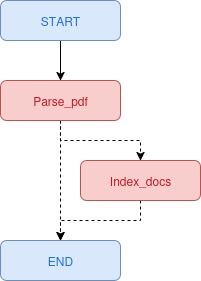
\includegraphics[width=0.3\linewidth]{static/schemas/indexGraph.drawio.png}
    \caption{Index graph structure}
    \label{fig:indexGraph}
\end{figure}

\textbf{Nodes:}\\

\paragraph{Parse pdf node}

This function scans a directory for PDF files, loads them using PyMuPDFLoader, splits the content into smaller chunks using RecursiveCharacterTextSplitter, and returns the processed documents. It filters out already processed files to avoid duplicates.

\begin{lstlisting}[caption={Parse pdf node}]
def parse_pdfs(
    state: InputIndexState, *, config: Optional[RunnableConfig] = None
) -> dict[str, str]:

    configuration = Configuration.from_runnable_config(config)
    
    path = Path(state.path)
    if not path.is_dir():
        raise FileNotFoundError(f"Directory not found: {state.path}")

    documents = []
    
    # Get new PDF files (excluding already processed ones)
    pdf_files = remove_duplicates(
        base=retrieval.get_existing_documents(),
        new=[str(p) for p in list(path.glob("*.pdf"))]
    )
    
    if not pdf_files:
        return {"docs": documents}
    
    #embeddings = load_embedding_model(model=Configuration.embedding_model, host=Configuration.ollama_host)

    text_splitter = RecursiveCharacterTextSplitter(
        chunk_size=4000,
        chunk_overlap=200,
        length_function=len,
        is_separator_regex=False
    )

    # Process each PDF file
    for pdf_file in tqdm(pdf_files, desc="Loading files..."):                
        # Load the file into a Document object
        if configuration.ocr:
            logger.debug("using server parser")
            loader = VisionLoader(
                file_path=str(pdf_file),
                mode = 'single',
                ollama_base_url= configuration.ollama_host,
                ollama_model=configuration.vision_model,
            )
        else:
            logger.debug("distant client not found, falling back to local parser")
            loader = PyMuPDFLoader(
                file_path=str(pdf_file),
                extract_tables='markdown',
                mode= "single"
            )
        
        # Split the Document content into smaller chunks
        document = text_splitter.split_documents(loader.load())
        #ensure metadata
        document[0].metadata={"source": pdf_file}
        # Add them to the list of Documents
        documents.extend(document)


    return {"docs": documents}
\end{lstlisting}

The following function is a conditional edge that skips the \texttt{index\_docs} node in case there are no documents to index.

\begin{lstlisting}[caption={Should index conditional edge}]
should_index(state: IndexState, *, config: RunnableConfig) -> str:

    if not state.docs:
        logger.info("No documents to index, ending workflow")
        return END

    return "index_docs"
\end{lstlisting}

\paragraph{Index documents node}

This function takes documents from the state, processes them in batches, and adds them to the configured retriever's index using the specified embedding model. After successful indexing, it signals for documents to be removed from the state.

\begin{lstlisting}[caption={Index doc node}]
def index_docs(
    state: IndexState, *, config: Optional[RunnableConfig] = None
) -> dict[str, str]:

    configuration = Configuration.from_runnable_config(config)
    
    # Prepare document batches
    documents_batch = make_batch(obj=state.docs, size= 20)

    # Index documents using the retriever
    with retrieval.make_retriever(
        embedding_model=load_embedding_model(model=configuration.embedding_model)
    ) as retriever:
        
        for i, batch in enumerate(tqdm(documents_batch, desc="Adding document batch..."), 1):
            retriever.add_documents(batch)

    return {"docs": "delete"} # To clear the value of the current thread
\end{lstlisting}

\textbf{Chunking Strategy}\\

The system supports two chunking approaches:

\begin{itemize}
    \item \textbf{Recursive Character Splitting}: Fixed-size chunks with overlap (4000 characters, 200 overlap)
    \item \textbf{Semantic Chunking}: Meaning-based division using embedding models (commented out for performance)
\end{itemize}

\begin{lstlisting}[caption={Text splitting configuration}]
text_splitter = RecursiveCharacterTextSplitter(
    chunk_size=4000,
    chunk_overlap=200,
    length_function=len,
    is_separator_regex=False
)
\end{lstlisting}

\textbf{Batch Processing:}
Documents are processed in batches of 20 to limit memory usage and provide progress feedback:

\begin{lstlisting}[caption={Batch processing implementation}]
documents_batch = make_batch(obj=state.docs, size=20)
for batch in tqdm(documents_batch, desc="Adding document batch..."):
    retriever.add_documents(batch)
\end{lstlisting}

\section{Retrieval System}

\subsection{Vector Store Management}

Homer utilizes ChromaDB as its primary vector store, providing persistent storage with cosine similarity search capabilities. The retrieval system implements a context manager pattern for resource management:

\begin{lstlisting}[caption={Vector store retriever implementation}]
@contextmanager
def make_retriever(embedding_model: Embeddings, **kwargs):
    vector_store = Chroma(
        collection_name=_COLLECTION,
        collection_metadata={"hnsw:space": "cosine"},
        embedding_function=embedding_model,
        persist_directory=VECTORSTORE_DIR,
    )
    yield vector_store.as_retriever(
        search_type="similarity_score_threshold", 
        search_kwargs={"k": 5, "score_threshold": 0.4}
    )
\end{lstlisting}

\subsection{Search Configuration}

The retrieval system supports multiple search strategies:

\begin{itemize}
    \item \textbf{Similarity Search}: Standard cosine similarity with configurable top-k results
    \item \textbf{Similarity Score Threshold}: Filters results below a minimum relevance threshold
    \item \textbf{Maximum Marginal Relevance (MMR)}: Balances relevance and diversity in results
\end{itemize}

\textbf{Default Parameters:}
\begin{itemize}
    \item \textbf{Top-k}: 5 documents per query
    \item \textbf{Score Threshold}: 0.4 minimum similarity
    \item \textbf{Collection}: "HOMER" with cosine similarity space
\end{itemize}

\subsection{Document Lifecycle Management}

The system provides comprehensive document lifecycle management through utility functions:

\begin{lstlisting}[caption={Document management functions}]
def get_existing_documents() -> list[str]:
    """Returns list of all indexed document sources"""
    
def delete_documents(docs: str | list[str]):
    """Removes documents by source filename"""
\end{lstlisting}

This enables users to manage their document collection, remove outdated content, and track indexing status through the web interface.\\

\paragraph{Get existing documents.}
The function \texttt{get\_existing\_documents} is used to list all the documents currently indexed in the ChromaDB vector store. More specifically, it returns the unique source file names associated with the stored documents. These source names are extracted from the metadata that is attached to each document. \\
This part of the code connects to the ChromaDB client and retrieves (or create if it does not exist) the "HOMER" collection. 
\begin{lstlisting}
client = get_chroma_client()
collection = client.get_or_create_collection(name=_COLLECTION, metadata=_COLLECTION_METADATA)
\end{lstlisting}
This line fetches all documents stored in the collection but includes only their metadata, not the actual content or embeddings
\begin{lstlisting}
results = collection.get(include=["metadatas"])
\end{lstlisting}

This block loops through the metadata and collects all values from the \texttt{"source"} field, which usually corresponds to the original file name. A set is used to ensure uniqueness (no duplicates).
\begin{lstlisting}
sources = set()
for metadata in results["metadatas"]:
if metadata and "source" in metadata.keys():
    sources.add(metadata["source"])
\end{lstlisting}

\paragraph{Delete documents.}
The function \texttt{delete\_documents} is used to remove one or multiple documents from the ChromaDB collection based on their source filename. This is useful for deleting outdated or incorrect files that were previously indexed.

Before deletion, the function ensures that the input is a list, even if the user passed a single string. This provides uniform handling.
\begin{lstlisting}
if isinstance(docs, str):
docs = [docs]
\end{lstlisting}

Then, for each source name in the list, the function deletes all documents that have a matching \texttt{"source"} field in their metadata.
\begin{lstlisting}
for doc_source in docs:
collection.delete(where={"source": doc_source})
\end{lstlisting}


\subsection{Experimental Support: Hybrid Retrieval with Milvus}

Homer also included an \textbf{experimental} backend using \textbf{Milvus Standalone}, a high-performance, embedded vector database available on Linux and macOS. Although not yet part of the stable release, this prototype demonstrates how Milvus can support hybrid search capabilities.

Milvus lite does not support hybrid-search and is not available on Windows; hence, ChromaDB was chosen. Milvus would be relevant in the case of a shared database between users, that would be running on a server.\\
In the example below, we are building a retriever that allows hybrid-search between Dense (HNSW with cosine metric) and BM25 sparse search.

\begin{minipage}{\linewidth}
\begin{lstlisting}[caption={Milvus hybrid retriever}]
from langchain_milvus import Milvus, BM25BuiltInFunction
from langchain_core.embeddings import Embeddings

@contextmanager
def make_retriever(embedding_model: Embeddings, **kwargs):
    vector_store = Milvus(
        embedding_function=embedding_model,
        builtin_function=BM25BuiltInFunction(),  # Enable BM25 for sparse vectors
        vector_field=["dense", "sparse"],  # Dense embeddings + sparse BM25
        collection_name=_COLLECTION,
        connection_args={
            "uri": VECTORSTORE_DIR,  # Local file-based storage like ChromaDB
        },
        index_params=[
            {"metric_type": "COSINE", "index_type": "HNSW"},   # Dense index
            {"metric_type": "BM25", "index_type": "AUTOINDEX"} # Sparse index
        ]
        consistency_level="Strong",
        drop_old=False,  # Don't drop existing collection
    )
    
    # Configure retriever with hybrid search and score threshold
    yield vector_store.as_retriever(
        search_type="similarity_score_threshold",
        search_kwargs={
            "k": 5,
            "score_threshold": 0.4,
            # For hybrid search, you can also specify:
            "ranker_type": "weighted",  # Use weighted ranking
            "ranker_params": {"weights": [0.7, 0.3]},  # Dense: 0.7, Sparse: 0.3
        }
    )
\end{lstlisting}
\end{minipage}

\paragraph{Advantages of Milvus.}
\begin{itemize}
    \item \textbf{Quick Setup:} Fully embedded—no Docker, no remote server
    \item \textbf{Hybrid Search:} Combines semantic and keyword-based retrieval
    \item \textbf{Scalable:} Designed to scale up to billions of vectors
    \item \textbf{Modular Integration:} Compatible with Homer's existing architecture
\end{itemize}

This experimental integration highlights the extensibility of Homer's architecture. In the future, a parallel \texttt{server\_retrieve} node could be a possibility, to search for additional context in another knowledge base.

\section{Error Handling and Resilience}

\subsection{Comprehensive Error Management}

Each component implements robust error handling with degradation:

\begin{lstlisting}[caption={Error handling pattern}]
try:
    # Main processing logic
    response = model.invoke(messages, config)
    logger.info("Operation completed successfully")
    return {"result": response}
except Exception as e:
    logger.error(f"Error in operation: {str(e)}")
    # Fallback mechanism
    return {"result": fallback_response}
\end{lstlisting}

\subsection{Logging Architecture}

The system implements structured logging with configurable levels:

\begin{lstlisting}[caption={Logging implementation}]
setup_logging("INFO")

# Usage across components
logger = get_logger(__name__)
\end{lstlisting}

\textbf{Log Levels and Usage:}
\begin{itemize}
    \item \textbf{INFO}: System status, configuration changes, major operations
    \item \textbf{DEBUG}: Detailed operation traces, parameter values, intermediate states
    \item \textbf{WARNING}: Non-fatal issues, fallback activations
    \item \textbf{ERROR}: Failed operations, exceptions with context
\end{itemize}

\subsection{Caching Strategy}


\begin{itemize}
    \item \textbf{Model Loading}: Models are cached within session state to avoid recompilation
    \item \textbf{Vector Store}: ChromaDB provides built-in caching for embedding lookups
    \item \textbf{Configuration}: Static configuration loading with dynamic host resolution
\end{itemize}

This architecture ensures optimal performance while maintaining system reliability and user experience quality.




\chapter{Vision Parser}

\section{VisionLoader}

Homer implements a dual-path document parsing system supporting both traditional text extraction and advanced vision-based processing. The parser architecture is designed around the \texttt{VisionLoader} class, which extends LangChain's \texttt{BaseLoader} interface.

\begin{figure}[H]
    \centering
    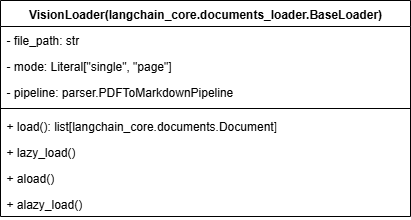
\includegraphics[width=0.55\linewidth]{static/schemas/classDiagramVisionLoader.drawio.png}
    \caption{Class diagram of the vision loader}
    \label{fig:VisionLoader}
\end{figure}

The vision parser is a loader based on Langchain's BaseLoader. It leverages a custom vision parser pipeline described later.\\

\begin{minipage}{\linewidth}
\begin{lstlisting}[caption={VisionLoader class structure}]
class VisionLoader(BaseLoader):
    def __init__(self, file_path: str, ollama_model: str, 
                 ollama_base_url: str, mode: Literal['single','page'] = 'page'):
        # Configuration and pipeline initialization
        self.pipeline = parser.PDFToMarkdownPipeline(
            ollama_model=ollama_model,
            ollama_base_url=ollama_base_url,
            enable_validation=False,
            dpi=400
        )
\end{lstlisting}
\end{minipage}

\section{Multi-Modal Parsing Architecture}

The multi-modal parser uses an Ollama LLVM to extract content from PDF documents, particularly effective for documents containing complex layouts, tables, mathematical formulas, and embedded images. In the current release, we use \texttt{Qwen2.5vl}. The implementation uses the following pipeline:

\begin{enumerate}
    \item \textbf{Page Rasterization}: PDF pages are converted to high-resolution PNG images (default 400 DPI)
    \item \textbf{Vision Model Inference}: Each page image is processed by the configured vision model
    \item \textbf{Content Extraction}: The model outputs markdown-formatted text preserving structure
    \item \textbf{Content Validation}: The model output is compared to the \texttt{fitz} text extraction to ensure that there are no significant data loss. (Not used in the current release)
\end{enumerate}

\begin{figure}[H]
    \centering
    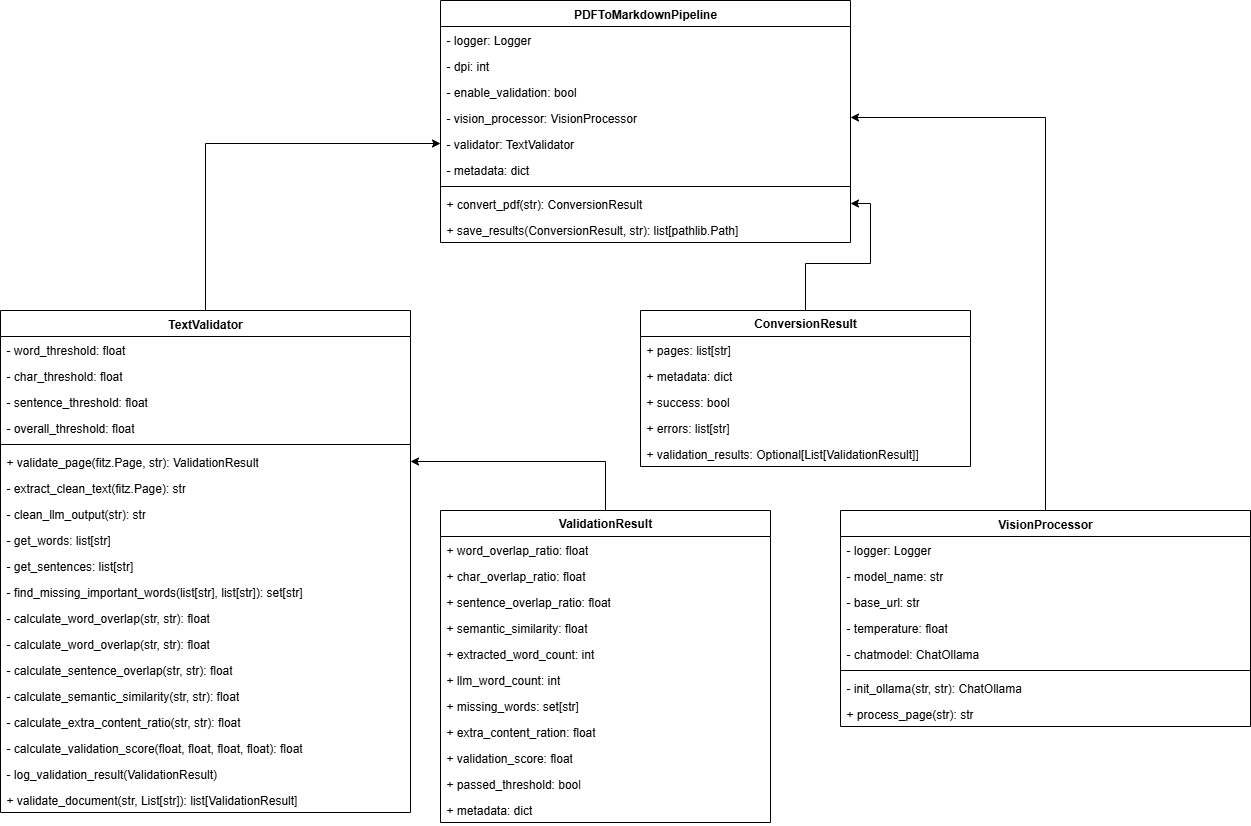
\includegraphics[width=\linewidth]{static/schemas/classDiagramOllamaVisionParser.drawio.png}
    \caption{Class diagram of the vision parser}
    \label{fig:VisionParser}
\end{figure}

The vision parser pipeline has been built using \texttt{Claude Sonnet 4} extensively.

\section{Text Validation System}

The parser includes a comprehensive validation system (\texttt{src/parser/validation.py}) that compares vision model output against traditional PyMuPDF text extraction. This dual-validation approach ensures accuracy and identifies potential extraction errors.

\textbf{Validation Metrics:}
\begin{itemize}
    \item \textbf{Word Overlap Ratio}: Percentage of words correctly extracted
    \item \textbf{Character Overlap Ratio}: Character-level accuracy using longest common subsequence
    \item \textbf{Sentence Overlap Ratio}: Structural preservation of sentence boundaries
    \item \textbf{Semantic Similarity}: Overall content similarity using normalized edit distance
\end{itemize}

The validation system calculates a weighted overall score:
\begin{equation}
V_{\text{score}} = 0.4 \times \text{Word Overlap} + 0.2 \times \text{Char Overlap} + 0.3 \times \text{Sentence Overlap} + 0.1 \times \text{Semantic Similarity}
\end{equation}

\subsection{Fallback Mechanism}

When vision parsing is disabled in the runnable config, the system falls back to PyMuPDF text extraction with table markdown support:

\begin{lstlisting}[caption={Parser fallback mechanism}]
if configuration.ocr:
    loader = VisionLoader(file_path=str(pdf_file), ...)
else:
    loader = PyMuPDFLoader(
        file_path=str(pdf_file),
        extract_tables='markdown',
        mode="single"
    )
\end{lstlisting}

This ensures consistent functionality across different deployment scenarios while optimizing resource utilization.




\begin{thebibliography}{9}

\bibitem{berge2025specifications}
Florent Bergé \& Mathieu de la Barre, 
\textit{Homer specifications}, 
SCK CEN, 05/2025

\bibitem{aliouat2025rag}
Raouf Aliouat, Rob Baby, Prabal Deb, Chad Kittel, Ritesh Modi, Ryan Pfalz \& Randy Thurman, 
\textit{Design and develop a RAG solution}, 
Microsoft Azure, 01/09/2025

\bibitem{berge2025hybrid}
Florent Bergé \& Mathieu de la Barre, 
\textit{Hybrid search for milvus}, 
SCK CEN, 09/05/2025

\end{thebibliography}

\end{document}